\documentclass[12pt]{article}
        \usepackage{graphicx,type1cm,eso-pic,color}
        \usepackage{hyperref}
        \usepackage[left=3.0cm,right=3.0cm,top=2cm,bottom=2cm,headheight=13.6pt]{geometry}
        \usepackage{subfigure}

\makeatother


\title{Review of the analysis note\\
Direct photoproduction of narrow baryon resonance in the reaction
$\gamma p\to pK^0 \bar K^0$ in CLAS
}

\author{
V. Kubarovsky (vpk@jlab.org)\\
}

\date{\today} 


\begin{document}
\maketitle{}

%%%%%%%%%%%%%%%%%%%%%%%%%%%%%%%%%%%%%%%%%%%%%%%%%%%%%%%%%%%%%%%
\newpage
   \section{vpk}
\begin{itemize}
\item The analysis note was written on June 17, 2013, 9 yeas ago.
In general, this analysis note is too short (20 pages only) and does not contain many necessary details that are needed to claim the existence of a pentaquark. The low level distributions, such as momentun, angles of all particles in data and Monte Carlo are absent. The calculation of the acceptance is completely missing.
\item Fig.~5. What are the cuts for this picture? Is it for $K_S$ or for $(\pi^+\pi^-)$?
\item Fig.~6. One dimensional projections needed. Better $M(p\pi^+\pi^-)$ and $M_X(\pi^+\pi^-)$.
\item Fig.~6. It is typical example of cut's selection to grow the peak.
\item Fig.~7. No justification for this cut is given exempt the visibility of the peak near 1.55 GeV.
\item Fig.~8. DOCA2 cut looks strange for me. It is less than DOCA1 but DOCA1 has more narrow distribution.
\item Fig.~8. Decay distnce look also very suspicious. Why does It go to zero at distance=0?
\item Fig.~9. The distributions are very similar. Why do we need cut at 1 cm?
\item Fig.~10. Looking to the DOCA2 distribution in Fig.~8 I would like to say that  even 1 cm cut is too tight. Analysis is using 0.5 cm.
Again, it seems to me that  the authors are choosing the cut where the signal is looking better.
\item Fig.~11. The choose of the parameter "d" is adequate. 
\item Fig.~12. Misprint: decay distance $\to$ collinearity angle, $\theta_C$.
\item No discussions of the Fig.~11-14 at all.
\item Fig.~15. It is not clear how the number of background events were estimated. By eye this number is around 200, pictures shows 114 events.
\item Chapter 6 "Data sampling". I don't think that the sampling of data tests the hypotheses of the resonance existence. It proves mostly that the data itself are stable during the experiment.
\item Page 17. Misprint: Fig.~7 $\to$ Fig.17. There are two more incorrect reference to Fig.~7 at the same page.
\item  Page 17.  "The fact that entire distribution outside of the peak drops significantly gives further confidence that the observed peak is real". Where is this statement coming from?
\item Chapter 8. "The $M(pK_S)$ invariant mass". Half a page of the text in this chapter doesn't give the scientific prove of the existence the structure in the $M(pK_S)$ mode.
\item Page 19, line 2. Misprint. $M(pK_S \to M(pK_S)$.
\item Fig.~ 20. The picture 20.b is different from the Fig.13 in the draft of the paper. In addition Fig.~13 capture is wrong: $M_X(K_S)\to M(pK_S)$. 
\item Chapter 8. Acceptance correction is not described at all. How was it done?
\end    {itemize}

\newpage
\section{Historical example of my analysis of the  search the pentaquark via interference with $\phi$-meson}
Below I presented some pictures from my parallel analysis that I made by Moskov's request for the search the pentaquark via interference with $\phi$-meson.
I was given the ODU cuts that were applied by the ODU group to 
claim the existence of the resonance. I followed exactly the ODU analysis chain and  found no signal.

It is interesting to note that the number of pentaquark events in the direct photoproduction and via interference with $\phi$-meson is approximately the same.


\begin{figure}[h!]
\center
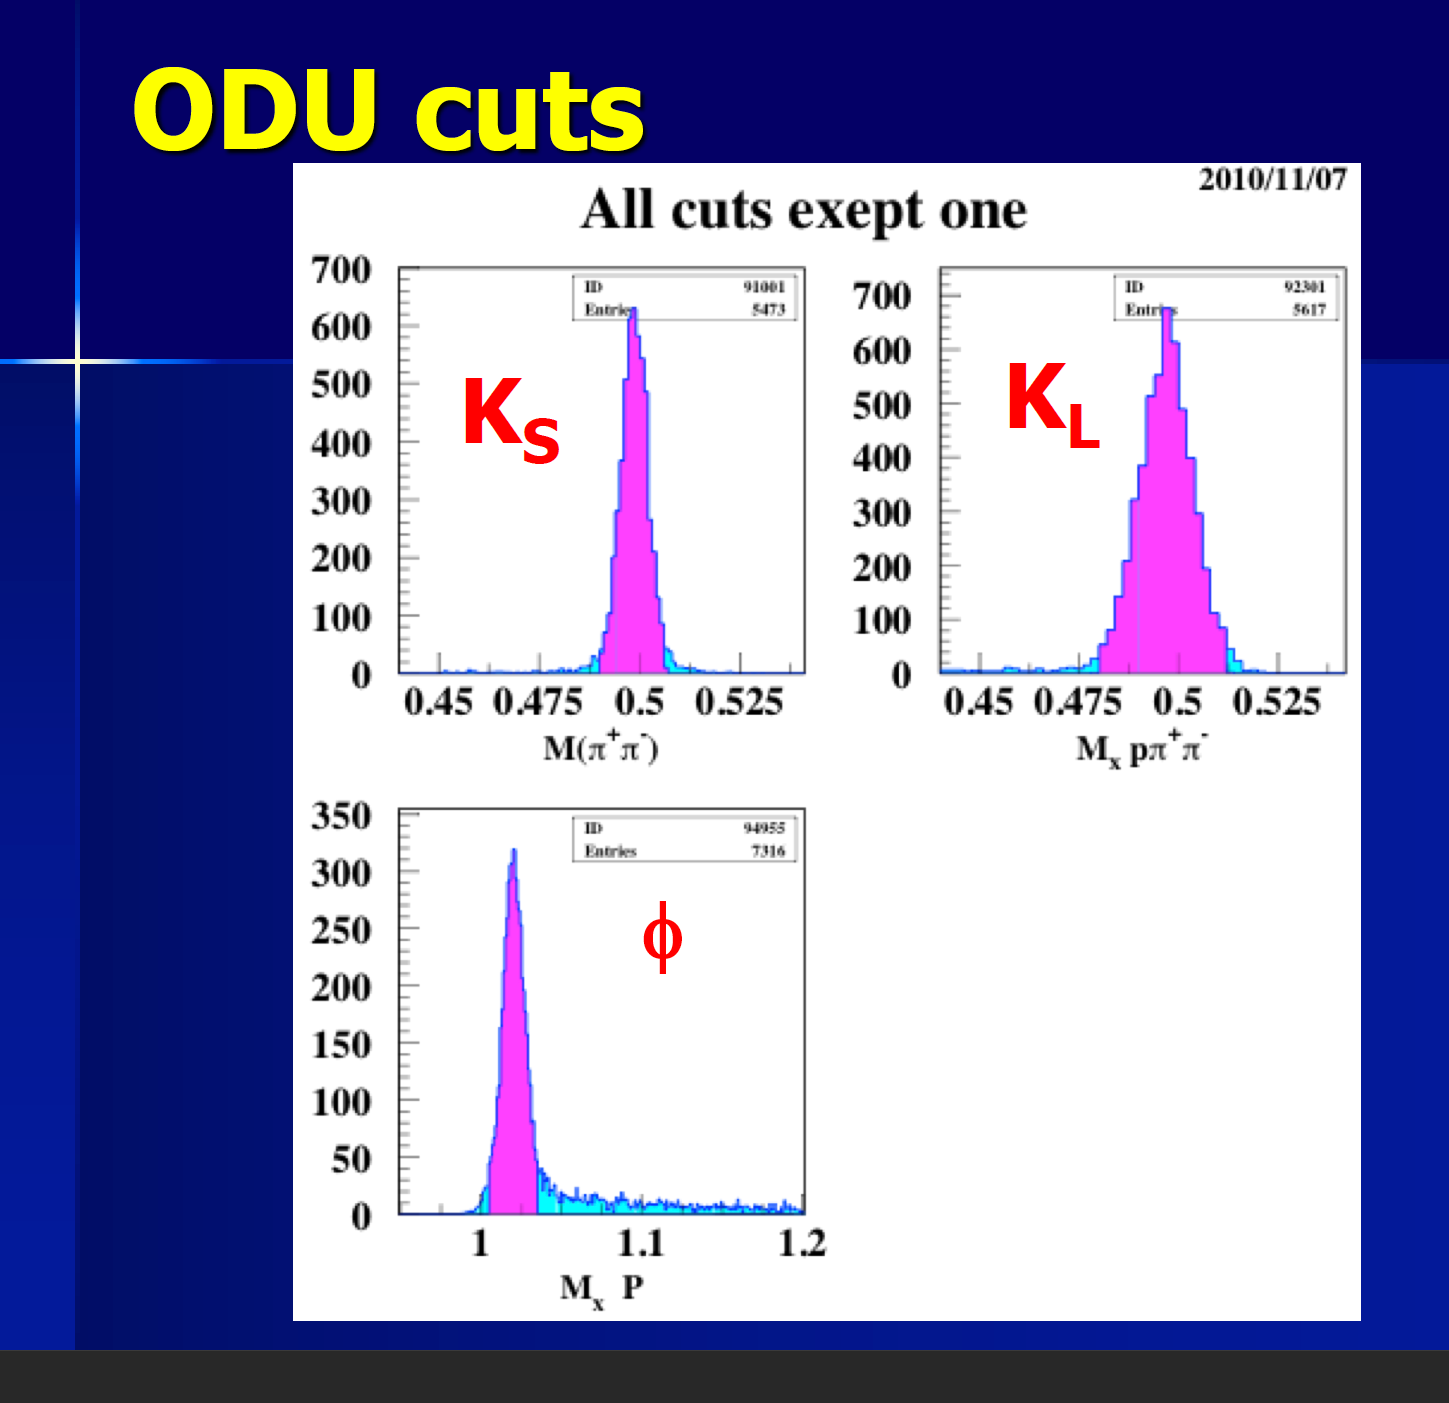
\includegraphics[width=0.4\textwidth]{KS_KL_phi.png}
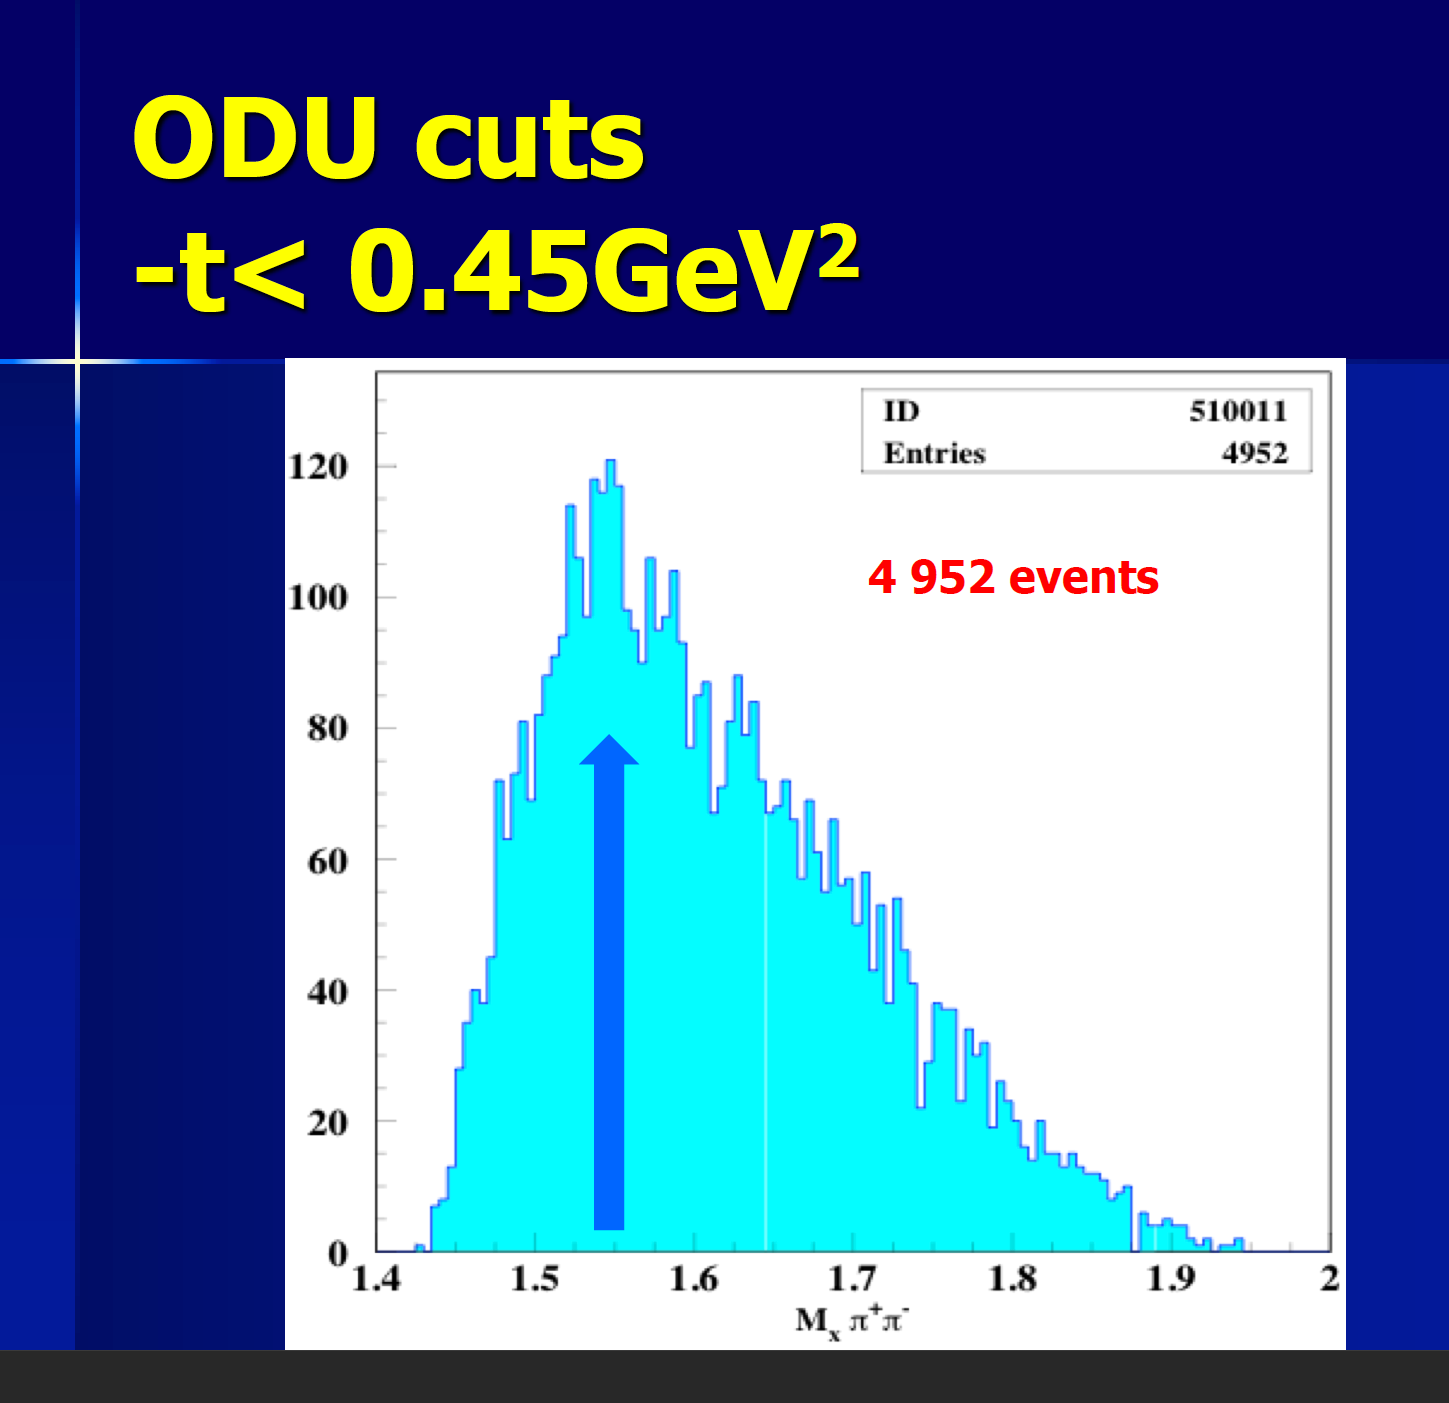
\includegraphics[width=0.4\textwidth]{Mx_pi+pi-.png}
\caption{ \label{fig:vpk} vpk analysis of the $\phi$-penta interference using ODU cuts.}
\end{figure}

\begin{figure}[h!]
\center
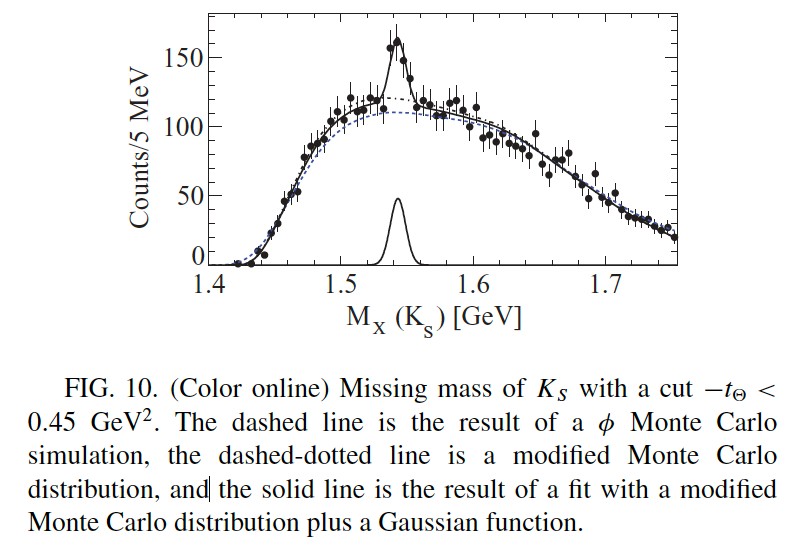
\includegraphics[width=0.8 \textwidth]{Mx_pi+pi-_PRC.png}
\caption{ \label{fig:PRC} Published in PRC C85, 035209 (2012).}
\end{figure}
\end{document}

\end{document}

%%%%%%%%%%%%%%%%%%%%%%%%%%
\begin{figure}[h!]
\center
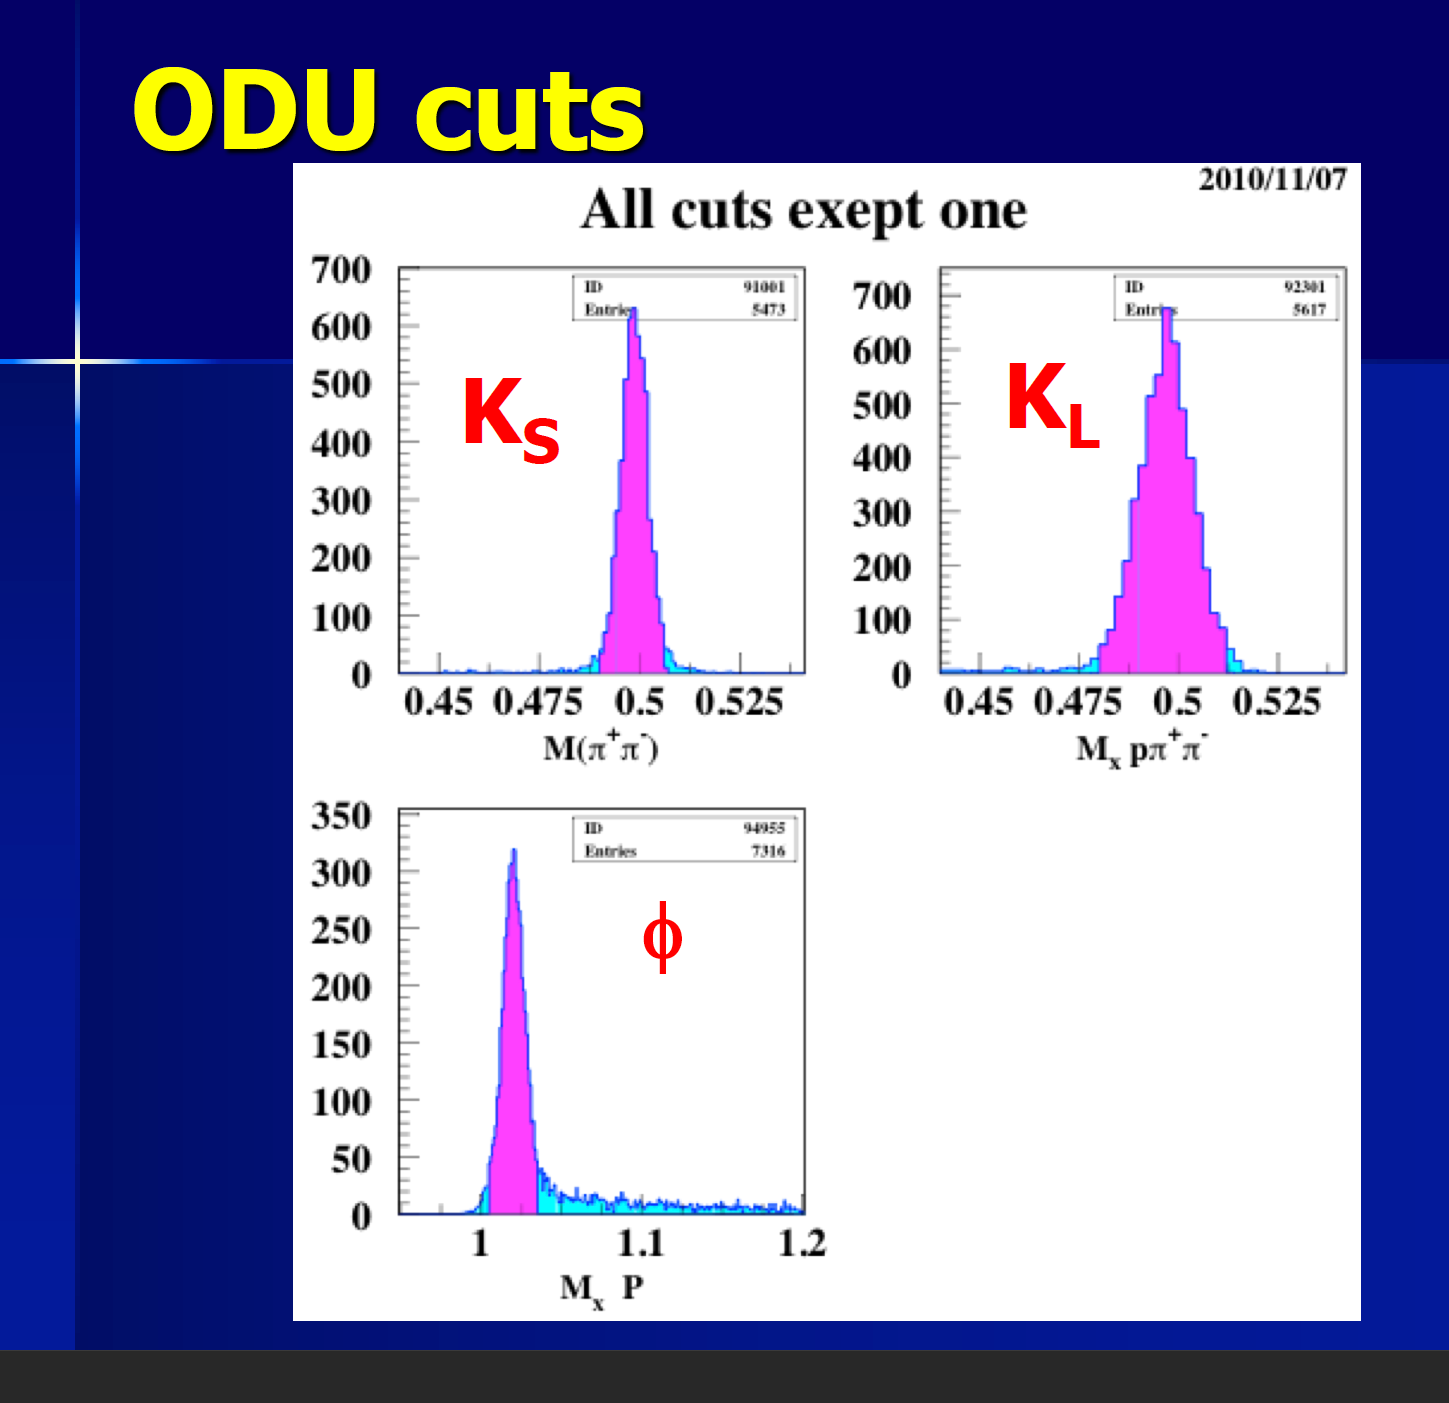
\includegraphics[width=0.53\textwidth]{KS_KL_phi.png}
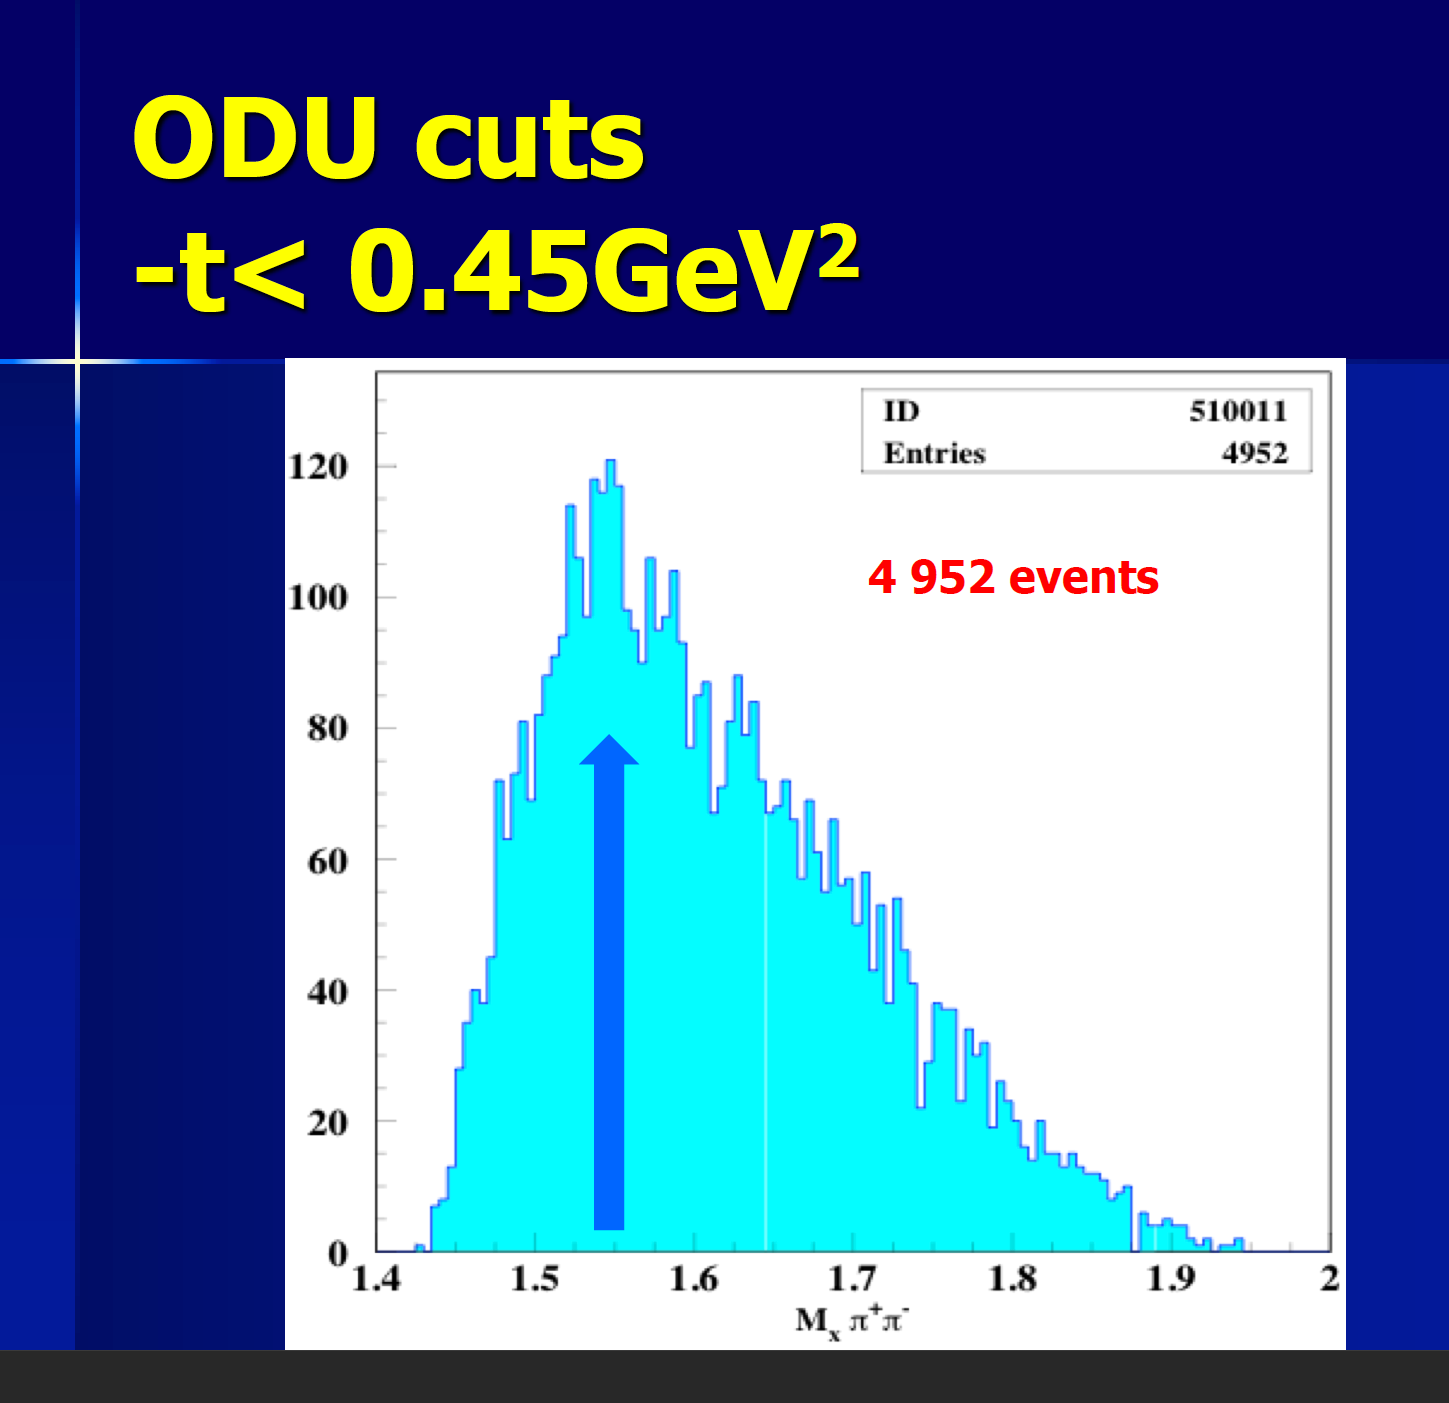
\includegraphics[width=0.46\textwidth]{Mx_pi+pi-.png}
\caption{ \label{fig:RICH_outer} ODU - vpk analysis of the ODU $\phi$-penta interference.}
\end{figuipaper draft Fig. 